\documentclass[tikz,border=10pt]{standalone}
% Load calc library for the $(Q)+(...)$ right-angle mark coordinates
\usetikzlibrary{calc}
% Scale s = 0.008538 units/px, origin shifted to B for readability (y flipped)
\begin{document}
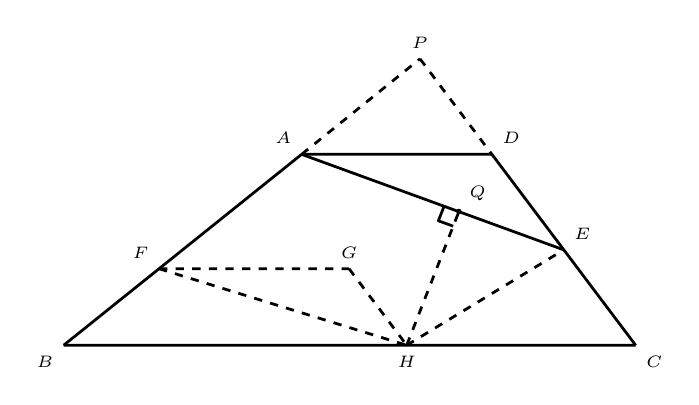
\begin{tikzpicture}[line width=1.0pt, line join=round]
  % Named points (converted from pixel coordinates)
  \coordinate (B) at (0.0004329005304350986,0.0005953554333522071);
  \coordinate (H) at (4.35687581395004,0.0003643742683936413);
  \coordinate (C) at (7.264394978067257,0.00021021589262359974);
  \coordinate (A) at (3.022304525707572,2.4249019878261597);
  \coordinate (F) at (1.2112774717509054,0.9724316506414472);
  \coordinate (E) at (6.351779934373237,1.211878723408266);
  \coordinate (Q) at (5.0199628786950266,1.6988981103861256);
  \coordinate (D) at (5.438994518819169,2.424773853501655);
  \coordinate (G) at (3.6251241684493025,0.9723036670701906);
  \coordinate (P) at (4.525852809657056,3.6376420615717855);

  % Solid segments
  \draw (B) -- (C);
  \draw (B) -- (A);
  \draw (A) -- (D);
  \draw (D) -- (C);
  \draw (A) -- (E);

  % Dashed segments
  \draw[dashed] (A) -- (P);
  \draw[dashed] (P) -- (D);
  \draw[dashed] (F) -- (G);
  \draw[dashed] (G) -- (H);
  \draw[dashed] (F) -- (H);
  \draw[dashed] (H) -- (Q);
  \draw[dashed] (H) -- (E);

  % Right-angle mark at Q (between QA and QH), side 0.2
  \draw ($(Q)+(-0.1879955230320336,0.06801044607734075)$) -- ($(Q)+(-0.26073612089319553,-0.11809102475576272)$) -- ($(Q)+(-0.07274059786116194,-0.18610147083310324)$);

  % Vertex dots/labels
  \fill (Q) circle (1pt);
  \node[above left, font=\fontsize{6}{7.2}\selectfont] at (A) {$A$};
  \node[above right, font=\fontsize{6}{7.2}\selectfont] at (D) {$D$};
  \node[above right, font=\fontsize{6}{7.2}\selectfont] at (E) {$E$};
  \node[above left, font=\fontsize{6}{7.2}\selectfont] at (F) {$F$};
  \node[above, font=\fontsize{6}{7.2}\selectfont] at (G) {$G$};
  \node[below, font=\fontsize{6}{7.2}\selectfont] at (H) {$H$};
  \node[below left, font=\fontsize{6}{7.2}\selectfont] at (B) {$B$};
  \node[below right, font=\fontsize{6}{7.2}\selectfont] at (C) {$C$};
  \node[above right, font=\fontsize{6}{7.2}\selectfont] at (Q) {$Q$};
  \node[above, font=\fontsize{6}{7.2}\selectfont] at (P) {$P$};
\end{tikzpicture}
\end{document}